\chapter{研究背景}

本研究を理解する上で必要な概念である, 強化学習とそのアルゴリズムであるMA-POCAの理論や,関連する研究について述べる.
また,本研究を行うことになった社会的背景についても述べる.

\section{津波避難誘導における課題}
本章では,我が国での津波避難誘導における課題について取り上げ,後述する提案手法の研究背景の理解を補助するものとする.\par 

災害大国である我が国において,地震発生後の津波避難誘導オペレーションは非常に重要である.
% TODO:津波避難オペレーションの重要性を述べる
また近年,津波以外にも異常気象等による気象災害の激甚化もあり,避難誘導の遂行にあたって,益々その危険性も増していると推察される.\par 

\subsection{訪日観光客数の増加と観光地における避難誘導の課題}
近年の大幅な観光客増加と,観光地における避難誘導の課題,その関連性について述べる.
\paragraph{我が国の観光客数増加}
我が国では,2007年にに観光立国推進基本法\footnote{議員立法により平成18年12月13日に成立し,平成19年1月1日から施行されている.本法律において,観光は21世紀における日本の重要な政策の柱として初めて明確に位置づけられた.}が施行され,国として観光客数の増加が進められてきた.
観光庁の調査によれば,我が国における訪日外国人観光客数は増加の一途を辿っている.下図は観光庁が公開している,2003年から2023年までの訪日外国人観光客数の推移を示したグラフである.
\begin{figure}[H] 
  \centering 
  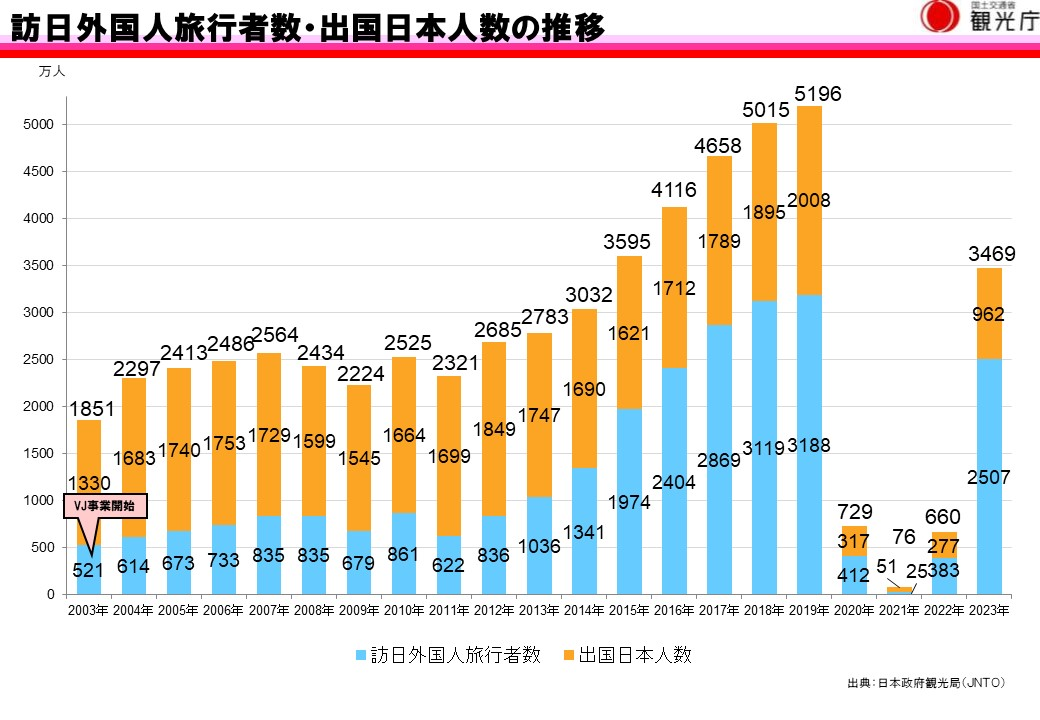
\includegraphics[width=0.8\textwidth]{Figures/001584918.jpg}
  \caption{2003年~2023年の訪日外国人旅行者数の推移} % TODO:いらないかも
  \label{fig:02} 
\end{figure}
上図を読み解くと,2003年から2019年にかけて,訪日外国人観光客数は倍以上に増加していることがうかがえる.2020年から2022年にかけては,著しく観光客数が減少しているが,これは新型コロナウイルスの世界的流行による影響であると考えられる.\par 
また,2023年は新型コロナウイルスによる行動自粛が解除されたことを受け,観光客数は2015年と同等水準まで回復しており,今後も増加するものと推察される.\par 
このような観光客数の急激な増加は,観光地の災害時の避難誘導タスクにおいて,以下のような問題を生じさせ適切な避難誘導を行えない可能性がある.
\begin{itemize}
  \item 観光客の土地勘がないため,的確な避難誘導が必要
  \item 観光客数は時間や季節によって変動するため,特定の避難所に多数の避難者が向かい,収容不足となる可能性がある.
  \item 避難誘導に従わずに周囲の人の動きに追従し,混乱を招く恐れがある.
\end{itemize}

このような,観光客の避難に関する問題は,多くの関連研究でも指摘されている.

\subsection{津波避難タワー・津波避難ビル}
我が国には,津波避難タワーや津波避難ビル\footnote{津波浸水が想定される地域において,地震発生時に住民が一時的,または緊急に避難・退避するための人工施設を言う.
内閣府が2005年に策定した「津波避難ビル等に係るガイドライン」に沿って進められ,2011年の東日本大震災\footnote{2011年3月11日14時46分頃に三陸沖の宮城県牡鹿半島の東南東130km付近を震源とする我が国最大規模の地震災害.}の発生を受け,「津波防災地域づくりに関する法律」によって津波防災対策が制度化された.}が建設されており,津波からの公的な避難先の1つとして提供されている.
\begin{figure}[H]
  \centering
  % 1枚目の画像
  \begin{subfigure}{0.45\textwidth}
      \centering
      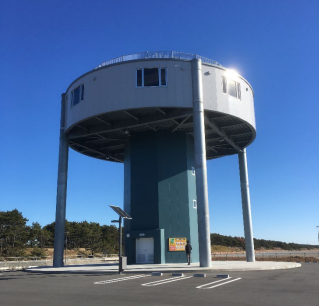
\includegraphics[width=\textwidth]{Figures/ShizuokaTunami-Tower.png}
      \caption{静岡県磐田市の津波避難タワー}
      \label{fig:image1}
  \end{subfigure}
  % 2枚目の画像
  \begin{subfigure}{0.5\textwidth}
      \centering
      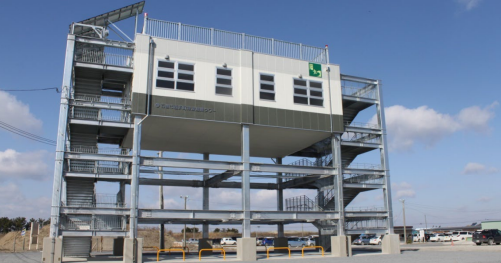
\includegraphics[width=\textwidth]{Figures/Isinomaki-TunamiBuild.png}
      \caption{宮城県石巻市の津波避難ビル}
      \label{fig:image2}
  \end{subfigure}
  \caption{実際の津波避難ビルと津波避難タワー}
  \label{fig:side_by_side}
\end{figure}
このような施設の建設にあたっては,避難経路や避難時間などの基準が国から示されており,自治体により適切な位置に建設が進められている.
特に,観光地では景観等の問題から,十分な高さの堤防や防波堤を用意することが難しいといった問題もあり,津波避難対策を強化する施策としてこのような津波避難施設の設置が自治体を主導に行われている.
このような施設は,津波から命を守る手段として非常に重要であるが,
避難者の行動,配分によっては収容定員を超過し,適切な避難が行えない可能性があることが示されている\cite{shimauchi2017}.\par 

しかし,その母数が足りず想定される避難者の数をカバーしきれない等の指摘や,被害予測の改訂等で必要な高さ等の基準を満たせていない等の問題も存在する\cite{yamada2018}.
加えて,ほとんどの観光客は土地勘がないとともに,防災意識もあまり高いとは言えない結果がアンケート調査で判明している.\cite{Okayasu2007}.

このような状況下では,近隣の高台へ避難することが求められるが,土地勘のない観光客や外国人観光客に対してこれを求めるのはかなり難しく,既往研究の多くで指摘されている問題である.\par 

また,観光地特有の問題として一部の避難所に避難者が集中し,避難完了時間が遅くなるというシミュレーション結果が示されており,適切に他の避難所(ないしは避難ビル)に避難者を誘導することの必要性が指摘されている\cite{kitahara2013tsunami}.


\vspace{\baselineskip}
以上の背景から,今後発生しうる,南海トラフ地震などの巨大地震とそれにより発生する津波からの避難に関して,その対策は進められてきてはいるものの,地元住民だけでなく観光客も含めた避難に関しては多くの課題を残している現状がある.
また,避難する人だけでなく,避難者を適切な場所へ誘導する人員の安全確保にも課題が残されている.


\subsection{二次被害の発生}
津波避難誘導(あるいは,他の災害における避難誘導)においては,発災直後から二次被害にあう危険性が高い地域で活動しなければならないため,現場で誘導を行う警察や消防員等の安全確保が問題になっている.\par
\paragraph{風水害時における人的被害の特徴}
以下の引用\ref{quote-yamada},および図\ref{fig-yamada}は,我が国で発生した1969年から2018年までの災害を対象に,消防団員が殉職した事例を消防白書や新聞記事,既往研究などから把握し,殉職時の状況を分析した結果が,山田らの研究\cite{yamada2020}によって報告されており,これを引用して紹介する.
\begin{quote}
  図-3 より,津波は,出動 途上,水防作業中,避難中,避難誘導中,人命救助中に 殉職者を出したことがわかった.なかでも避難誘導中と 避難中を合わせると全体で約 80\%を占めており,避難に関係する時に殉職者が出ている.
  \begin{figure}[H] 
    \centering 
    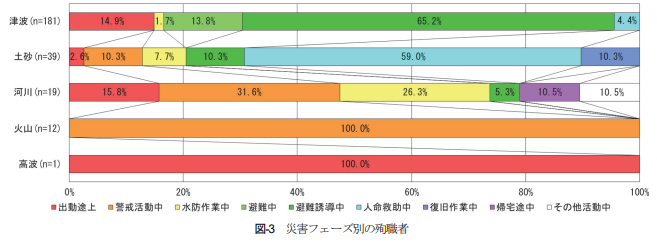
\includegraphics[width=0.8\textwidth]{Figures/fig-01.png}
    \caption{消防団員の災害フェーズ別殉職者の割合} 
    \label{fig-yamada}
  \end{figure}
  \label{quote-yamada}
\end{quote}
以上より,津波災害時の消防団員おけるの2次被害に関しては,避難誘導中が最も多い結果であることが示されている.上記は消防団員に限定した統計であるが,同じく避難誘導を行うすべての人員においても同様の傾向があると推察される.\par
また,東日本大震災のケースにおいても,避難誘導にあたった警察職員や自治体職員の多数が地域住民の避難誘導中に津波に巻き込まれ殉職された事例が報告されており\cite{npa2012}\cite{syouboukikin2012},このような二次被害の防止は避難誘導において重要な意味を持つ.

\section{既存のドローンの災害対応における活用事例と航空法改正}
加えて,我が国では,2022年に航空法が改正され,これまで規制されていたドローンの有人地帯目視外飛行(レベル4飛行\footnote{無人機の運用・操縦方法をレベル別に定めたもの.レベル4では操縦者が直接目視で機体を見ていなくても有人地帯でドローンを飛ばすことが可能になった.})が解禁された.
これにより,これまでドローンの活用が規制されていた防災分野での利活用や研究が大きく進んだ背景がある.\par 
\begin{table}[H]
  \centering
  \begin{tabular}{|l|lll|}
  \hline
       & 操縦方法 & 視界         & 飛行可能場所  \\ \hline
  レベル1 & 操縦飛行 & 目視内        & 無人/有人地帯 \\ \hline
  レベル2 & 自律飛行 & 目視内        & 無人/有人地帯 \\ \hline
  レベル3 & 自律飛行 & 目視外(補助者無し) & 無人地帯    \\ \hline
  レベル4 & 自律飛行 & 目視外(補助者無し) & 有人地帯    \\ \hline
  \end{tabular}
  \caption{ドローンの飛行レベル別概要}
\end{table}
近年我が国では,少子高齢化に伴う労働人口の減少の問題もあり,災害対応人材の不足が懸念されている背景がある.そのような人手不足に対応するため,ドローン等による災害対応の機械化・省人化が進められ始めている.
総務省・消防庁が公開しているデータ\cite{soumusho-01}によると,全国の消防本部におけるドローンの活用率は年々上昇しており,2017年には9.6\%だったものが,2021年には52.9\%と全国半数以上の消防本部でドローンの利活用が進めらたことが報告されている.

\subsection{ドローンによる避難誘導の先行研究と自治体の実証実験の事例}
ドローンを初めとするUAVの津波避難誘導に置ける活用方法を検討した既往研究が存在する。
杉安らの研究では、津波避難時の迅速な避難行動を促進するために、UAV(無人航空機)の活用可能性を示し,避難誘導を視覚的に行うことを目的とし、福島県いわき市を対象に実証実験を行っている\cite{sugiyasu2018uav}.

また、本研究と関連する先行研究事例として,鈴木らが行った協調ドローンを用いた避難誘導支援システムの研究がある\cite{suzuki2020drone}.この研究では,ドローンを活用して,安全な避難経路を生成し,被災者を誘導するシステムを提案している.
被災者はARマーカーを身に着け、ドローンがこれを識別することで位置情報を取得し,後述するa*アルゴリズムにより避難経路を探索し,計算した軌道情報に沿って対象者を誘導するものである.この研究では実機による誘導試験も行っており,ドローンによる避難誘導の実現可能性を示した。
もう一つの先行研究事例として、複数のドローンが連携して避難誘導を行うことを検証した高橋らの研究が存在する\cite{takahashi2018uav}。この研究では、自然災害時にUAV(無人航空機)を活用して避難誘導を行う支援システムの設計と試作について述べている.
このシステムは複数のUAVが連携して避難者を誘導する仕組みを構築しており、沿岸部地域を対象にした実証実験まで行っている. UAVエージェントによる避難誘導プラン生成と経路選択,複数の UAV の協調による避難誘導機能の実現可能性が示された.\par

また,改正航空法の施行後,沿岸部の自治体を中心に,津波避難誘導を行うドローンの研究や実証実験が進められている.
宮城県仙台市では,東日本大震災の際に津波避難誘導を行っていた自治体職員が津波に巻き込まれ犠牲になった事例を受け,津波避難を呼びかける手段として津波避難広報ドローンの研究が行われている\cite{sendai_tsunami_drone}.この実証実験は,「自動運航のドローンにより津波避難広報を行うこと」及び「専用のLTE通信網でドローンの制御等を行うこと」の2点において世界初の事例で,
Jアラート\footnote{全国瞬時警報システム(Jアラート)とは,弾道ミサイル情報,緊急地震速報,大津波警報など,対処に時間的余裕のない事態に関する情報を携帯電話等に配信される緊急速報システム}による津波情報を受信した後,飛行経路上の気象条件を確認し自律的にドローンの飛行可否を判断した後,事前に定められた飛行ルート上を飛行しながら津波避難のアナウンスを行うというものである.
また,ドローンの管制システムには専用のLTE通信網を利用しており,令和4年10月に整備を完了し本格運用に入っている.\par


以上の様に、ドローンを用いた避難誘導システムの基礎研究や、自治体による避難誘導案内ドローンの整備など、災害時の避難誘導においてドローンの活用が検討,実装が進められている。\par

ただし、これらの研究事例においては,後述する提案手法で示す,本研究が行うような要避難者の位置分布に基づいた各ドローンの配置や移動,避難先の収容人数を考慮した避難誘導の最適化は行われていない.
これらの点を後述する提案手法の章にて、本研究が示す新規性として具体的に述べる.

\section{強化学習}
強化学習とは,エージェント\footnote{モデルを訓練するための主体.環境に対して行動を出力する.}と環境\footnote{エージェントがいる世界,モデルの訓練を行うための様々な機能や状態を提供する.}との相互作用を通じ,
得られる報酬\footnote{エージェントの行動の良し悪しを判断する評価値.行動に対する環境からの評価}を最大化するエージェントの方策\footnote{ポリシーとも呼ばれる.環境の状態に基づいて,次の行動を決定するための
ルール}を学習する機械学習アルゴリズムの種類である.
\begin{figure}[H] 
  \centering 
  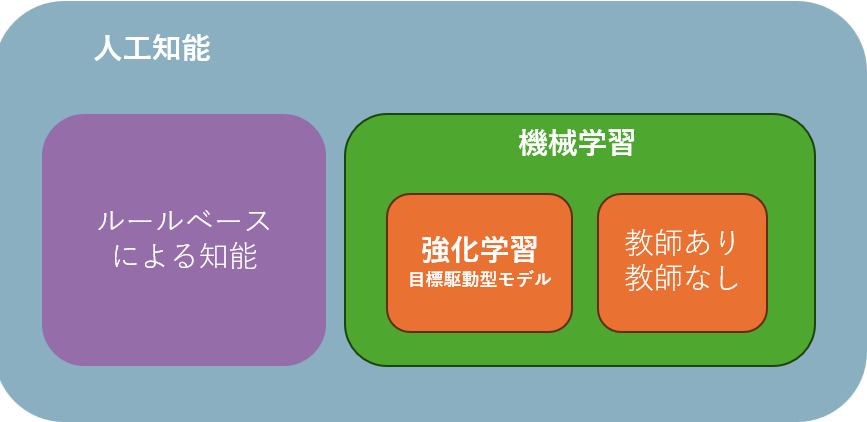
\includegraphics[width=0.6\textwidth]{Figures/2024-12-09 202235.png}
  \caption{強化学習の枠組み概念図} 
  \label{fig:01} 
\end{figure}
教師あり学習・教師なし学習のデータ駆動型機械学習モデルと異なり,事前に訓練データを作成する必要はなく,訓練に必要なデータはエージェントが環境から得るものである.強化学習は与えられた環境の中で,最適な戦略行動 (方策)を分析することが目的となる.
このような特性から,強化学習は目的駆動型モデルや行動駆動型モデルと呼ばれることもある.
エージェントの一連の流れである「観測」,「行動出力」,「報酬獲得」のサイクルを決定と呼ぶ.
\subsection{マルチエージェント強化学習の基本概念}

マルチエージェント強化学習 (Multi-Agent Reinforcement Learning, MARL) では,複数のエージェントが環境と相互作用し,それぞれが自身の行動方策を学習しながら,協調または競争を行う.以下にその基本的な数式を示す.

\subsection*{環境の定義}
環境は,部分観測可能マルコフ決定過程 (Decentralized-POMDP) として定義される:
\[
\mathcal{M} = \langle N, S, \{O_i\}_{i=1}^N, \{A_i\}_{i=1}^N, P, r, \gamma \rangle
\]
ここで:
\begin{itemize}
    \item $N$:エージェントの数
    \item $S$:環境の状態空間
    \item $O_i$:エージェント$i$の観測空間
    \item $A_i$:エージェント$i$の行動空間
    \item $P(s' | s, \boldsymbol{a})$:状態$s$と行動の組み合わせ$\boldsymbol{a} = (a_1, a_2, \dots, a_N)$から次の状態$s'$への遷移確率
    \item $r(s, \boldsymbol{a})$:共有報酬関数
    \item $\gamma$:割引率
\end{itemize}

\subsection*{エージェントの行動方策}
各エージェント$i$は,観測$O_i$に基づき行動を選択する方策$\pi_i(a_i | o_i)$を学習する.エージェント全体の方策は次のように表される:
\[
\pi(\boldsymbol{a} | \boldsymbol{o}) = \prod_{i=1}^N \pi_i(a_i | o_i)
\]

\subsection*{状態価値関数と行動価値関数}
\begin{itemize}
    \item 状態価値関数$V^\pi(s)$は,状態$s$から始まり方策$\pi$に従ったときの期待累積報酬である:
    \[
    V^\pi(s) = \mathbb{E}_\pi \left[ \sum_{t=0}^\infty \gamma^t r(s_t, \boldsymbol{a}_t) \mid s_0 = s \right]
    \]
    \item 行動価値関数$Q^\pi(s, \boldsymbol{a})$は,状態$s$で行動$\boldsymbol{a}$を取った場合の期待累積報酬である:
    \[
    Q^\pi(s, \boldsymbol{a}) = r(s, \boldsymbol{a}) + \mathbb{E}_\pi \left[ \sum_{t=1}^\infty \gamma^t r(s_t, \boldsymbol{a}_t) \right]
    \]
\end{itemize}

\subsection*{集中化されたCritic}
MARLでは,集中化されたCriticを用いて全エージェントの観測$\boldsymbol{o}$と行動$\boldsymbol{a}$を基に価値関数を近似する:
\[
Q^\pi(s, \boldsymbol{a}) = f_\phi(s, \boldsymbol{a})
\]
ここで$f_\phi$はパラメータ$\phi$を持つ関数近似器(通常はニューラルネットワーク)である.

\subsection*{Advantage関数}
アクター・クリティックアルゴリズムでは,Advantage関数を用いて方策の更新を行う:
\[
A^\pi(s, \boldsymbol{a}) = Q^\pi(s, \boldsymbol{a}) - V^\pi(s)
\]

\subsection*{方策の更新}
エージェントの方策は,Advantage関数を最大化するように勾配上昇法で更新される:
\[
\nabla_\theta J(\pi_\theta) = \mathbb{E}_{\pi_\theta} \left[ \nabla_\theta \log \pi_\theta(a | s) A^\pi(s, a) \right]
\]

\subsection*{協調と競争}
協調タスクでは,全エージェントがグループ報酬$r(s, \boldsymbol{a})$を最大化する.一方,競争タスクでは,各エージェントが自分の報酬を最大化する.

\subsection{MA-POCA(MultiAgent POsthumous Credit Assignment)}
  環境内のエージェントの個体数の増減に対応し,エージェント間の協調行動を重んじるようなタスクを学習するのに適しているアルゴリズムがMA-POCA(MultiAgent POsthumous Credit Assignment)\cite{mapoca}である.\par 
  MA-POCAは既存のマルチエージェントアルゴリズムと比較して,以下の特徴を持つ.
  \begin{itemize}
    \item 環境内のエージェント数の増減に対応した学習が可能
    \item エピソード内でエージェントが生成・消滅するタスクや,標準的な協調タスクにおいて,既存手法を大幅に上回る性能を示した
  \end{itemize}
  例えば,実世界で動くようなドローンをエージェントとして,その群衆飛行を考えた時,あるバッテリーが切れたり,故障したりすることが考えられ,エージェントが他のエージェントよりも先に行動不能(早期終了)になる場合が考えられる.
  既存のマルチエージェントアルゴリズムは,エージェントがエピソード\footnote{エージェントが環境と相互作用してタスクを完了するまでの一連のステップのこと.例えば,迷路のスタート地点からゴール地点までの移動がこれに該当する.一方,「ステップ」とは,そのエピソード内でエージェントが1回行動を選択し,環境から報酬と次の状態を受け取る単位時間のことである.}
  終了前に消滅した場合,そのエージェントの行動出力に関係なく状態を固定することでこれを再現する.これを吸収状態と言い,このようにすることでCriticへの入力数を固定したまま学習を行うことが出来るが,同時に無駄な情報を入力しているとも捉えることができ,環境内のエージェント数が多いほどこの問題は顕著に出現することが指摘されている.\par
  早期終了になったエージェントは,与えられたグループ報酬を経験することができない為,自身の行動のグループにおける価値を計算することができない.MA-POCAは,この問題を解消するために提案されたアルゴリズムで,エージェントが早期終了しても価値を伝搬させるアルゴリズムとなっている.\par
  \paragraph{MA-POCAの性能評価}
  MA-POCAは既存のMARL手法よりも多くの場合で性能が向上することが報告されている\cite{mapoca}.
  下記のような4つの実験環境において,マルチエージェント強化学習手法COMA\footnote{},そして,シングルエージェント強化学習手法PPO\footnote{}とMA-POCAの性能を比較した結果が示されている.
  \begin{figure}[H] 
    \centering 
    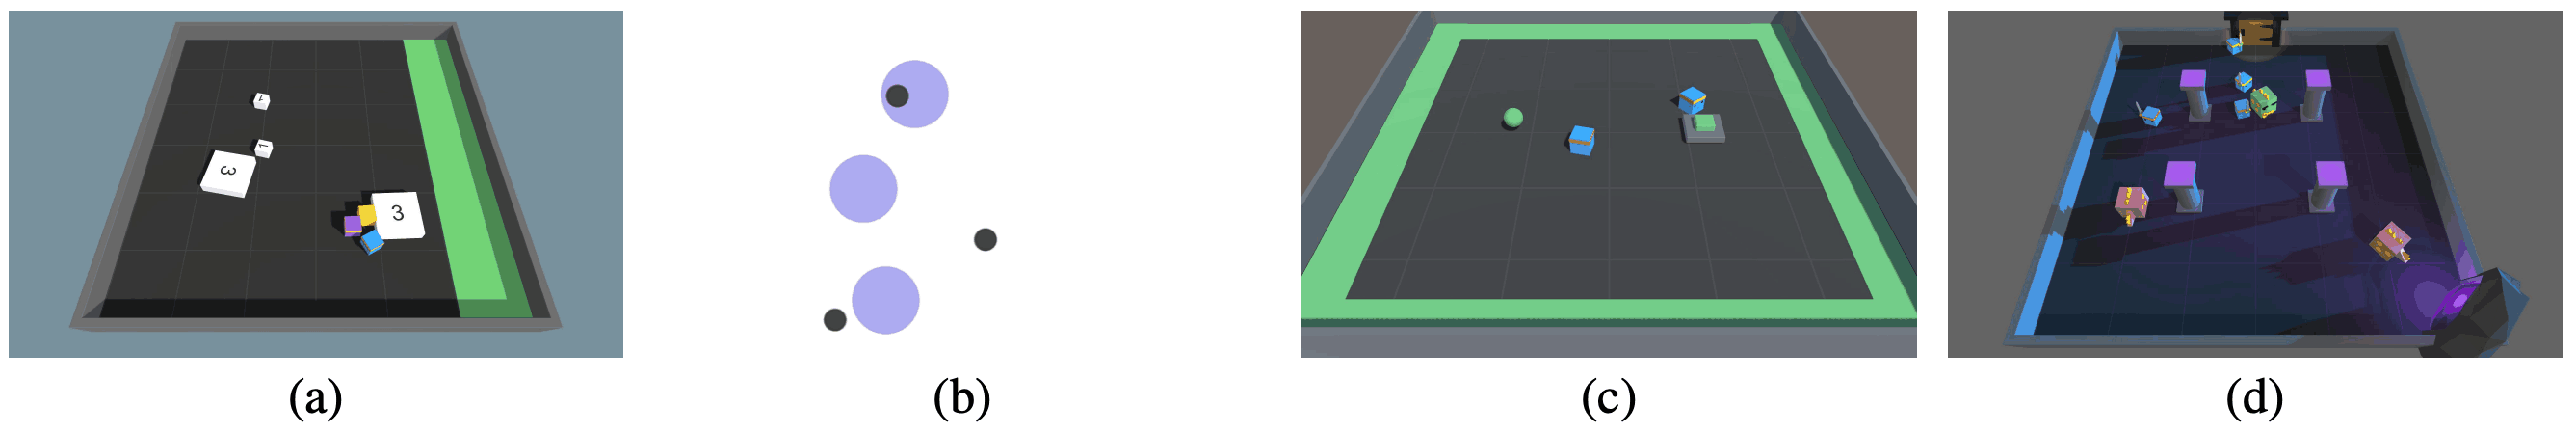
\includegraphics[width=1.0\textwidth]{Figures/2022-10-06_10.03.52.png}
    \caption{MA-POCAの性能評価を実施した環境} 
    \label{fig:01} 
  \end{figure}
  \begin{enumerate}[(a)]
    \item \textbf{Collaborative Push Block}
    エージェント(青,黄,紫)は白いブロックを緑の領域まで押す.大きなブロックはより多くのエージェントが押す必要がある.
  
    \item \textbf{Simple Spread}
    エージェント(紫)は互いにぶつかることなく,ターゲット(黒)をカバーするように移動しなければならない.
    
    \item \textbf{Baton Pass}
    青いエージェントが緑色のfoodをつかみ,緑色のボタンを押すと別のエージェントが生まれ,次のfoodをつかむことができるようになるので,それを繰り返す.
    
    \item \textbf{Dungeon Escape}
    青いエージェントは緑のドラゴンを倒し,そのうちの1人を犠牲にしてカギを出さなければならない.チームメイトは鍵を拾って,ピンクのドラゴンを避けながら,ドアまでたどり着くタスク.
\end{enumerate}
以下の引用図\ref{fig:MAPOCA}は,上記4環境における,累積報酬の推移を示している.このように,MA-POCAは既存のMARL手法よりも多くの場合で性能が向上することが報告されている.
\begin{figure}[H] 
  \centering 
  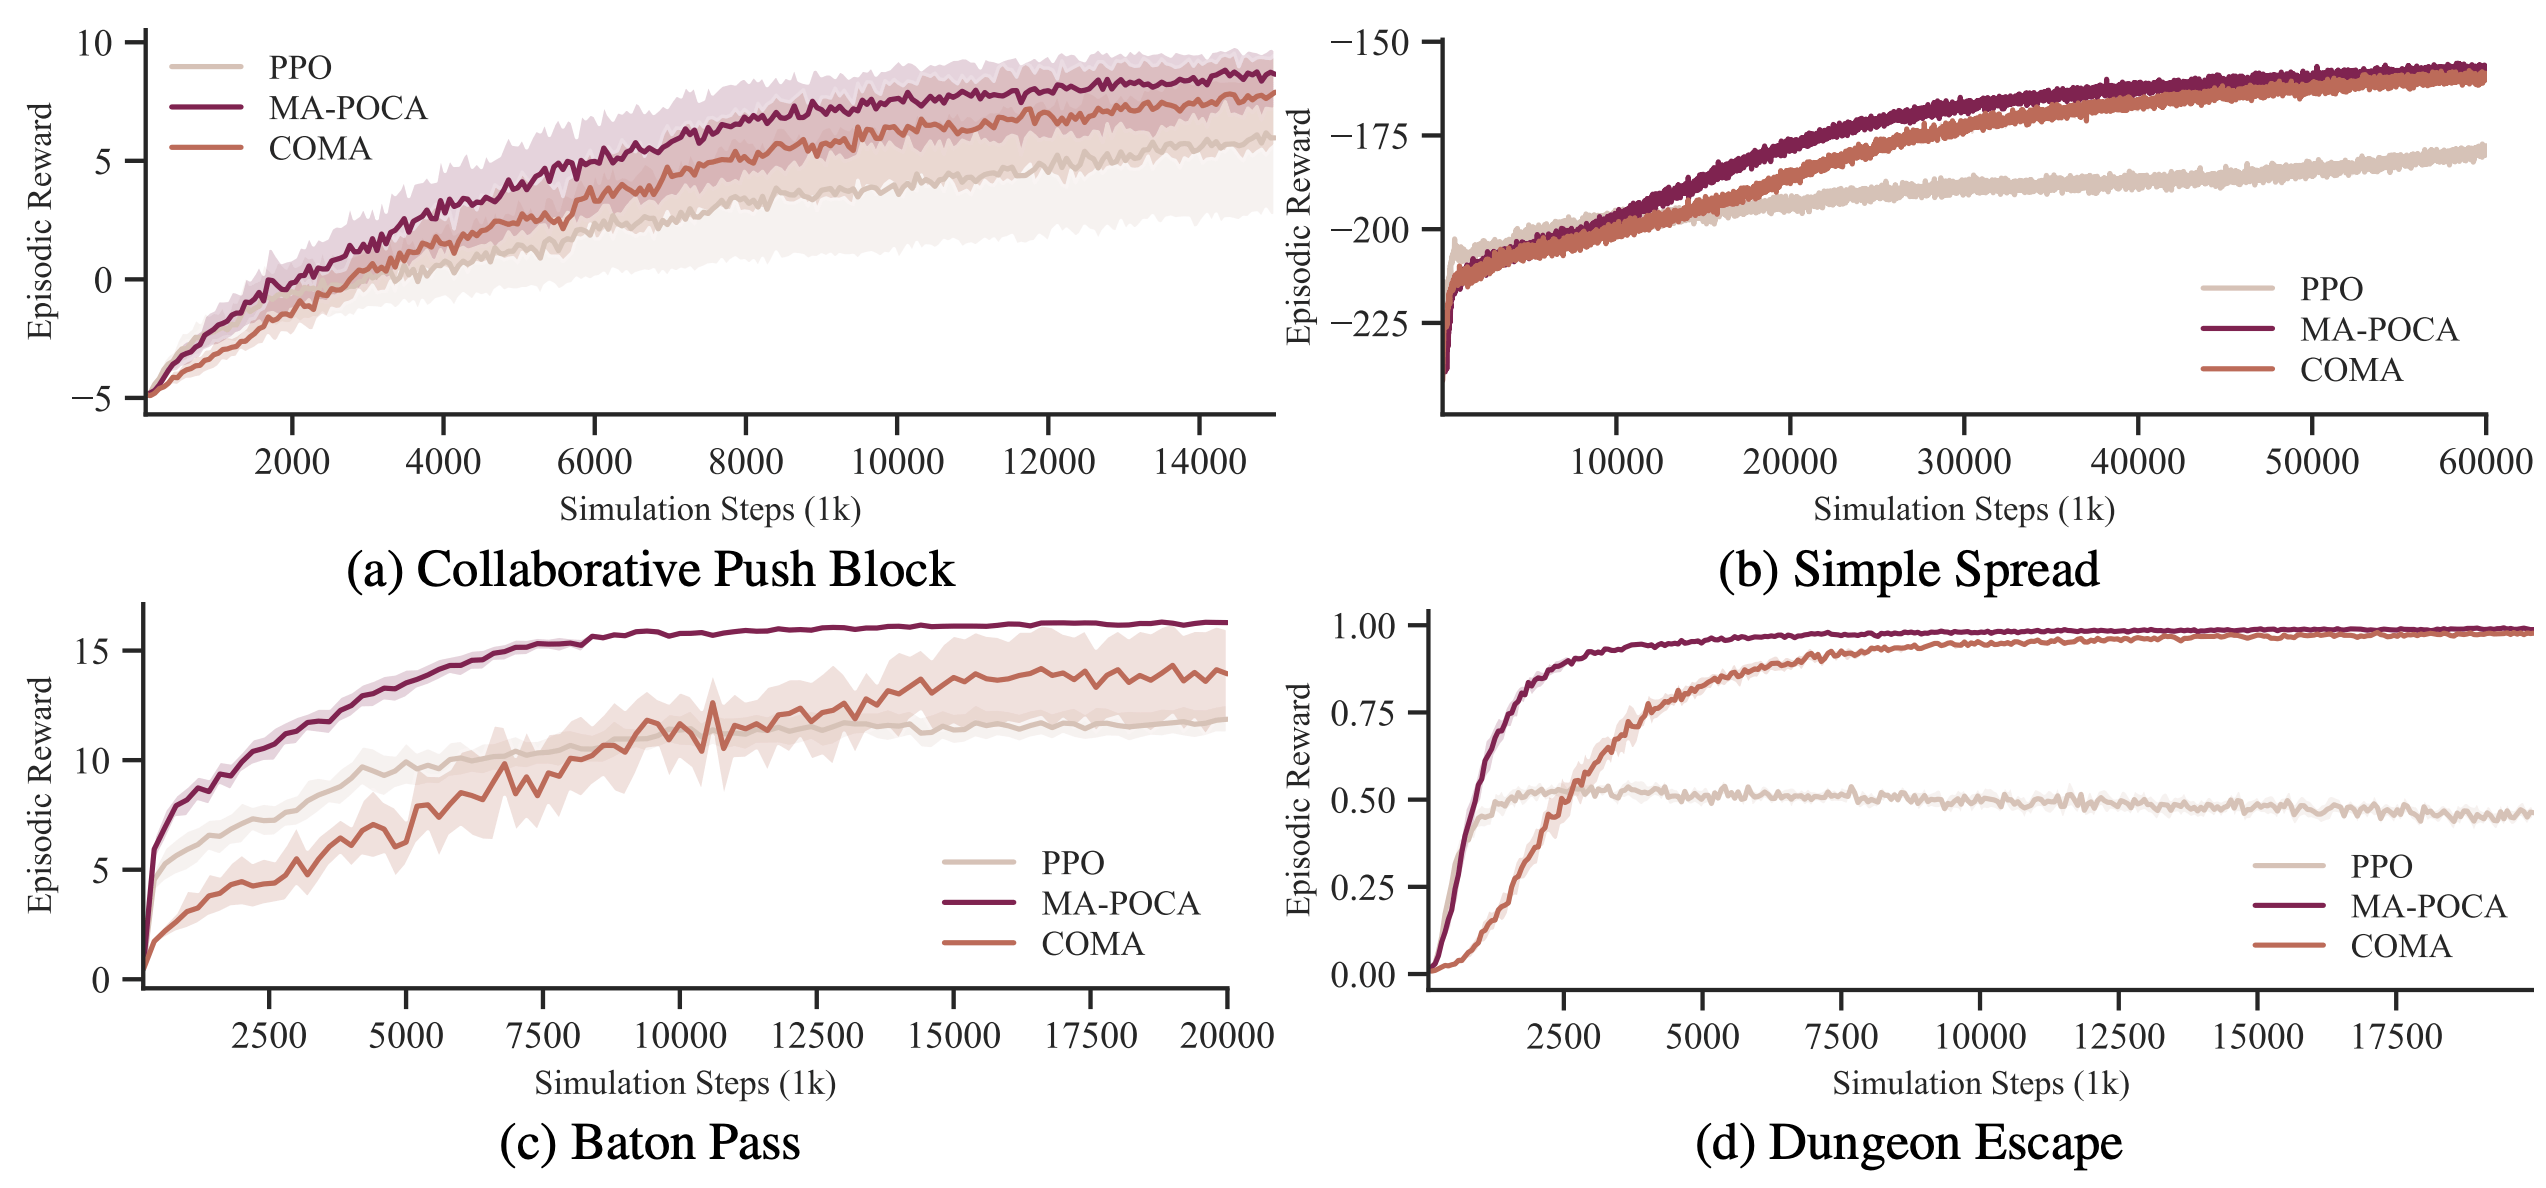
\includegraphics[width=1.0\textwidth]{Figures/2022-10-06_10.04.14-min.png}
  \caption{各環境でのMA-POCAの性能評価結果} 
  \label{fig:MAPOCA} 
\end{figure}

\section{ナビゲーションメッシュ}
デジタルゲームにおける人工知能\cite{miyake2016}には大きく3つの種類がある.
\begin{itemize}
  \item キャラクターAI : ゲームやシミュレーション内で使用するNPCの頭脳
  \item メタAI : ゲームやシミュレーション全体を監督し,難易度等を調整する
  \item ナビゲーションAI : キャラクターの移動経路検索や障害物等の管理を行う
\end{itemize}

本研究では,エージェントの経路探索に上記のナビゲーションAIに区分される,ナビゲーションメッシュと呼ばれる機能を利用する.
ナビゲーションメッシュは,ノード\footnote{このノードをウェイポイントデータと呼び,ダイクストラ法等のグラフ探索アルゴリズムを用いて最短経路を検索することが可能になる}の連結(グラフ)によって移動可能領域を覆うことで,キャラクターから移動可能範囲,経路を認識させるためのゲームAI技術である.\par
都市モデル上でエージェントを動かす場合,あらゆる経路や移動手段が考えられ,エージェントが移動可能な道路や領域,障害物として認識した上で行動するにはモデル訓練時の経験においてそれらを学習する必要がある.
本研究の目標は,エージェントが避難者を,誘導人数や収容人数等を考慮し適切な避難所へ誘導することが目標なため,ナビゲーションメッシュを使用し事前にエージェントが移動可能な範囲を定めるものとする.


\subsection{a* アルゴリズム}
キャラクターの移動経路を探索するナビゲーション機能のアルゴリズムとしてはa*アルゴリズムが広く利用されている.
a*アルゴリズムは,最短経路を探索するためのグラフ探索アルゴリズムで,経路をノードとして表現しグラフ探索を行う.

スタートノードからゴールノードまでの最短経路を探索する際に,次の評価関数$f(n)$を用いる:
\[
f(n) = g(n) + h(n)
\]
ここで:
\begin{itemize}
    \item $f(n)$: ノード$n$の総評価値.スタートからゴールまでの推定コスト.
    \item $g(n)$: スタートノードから現在のノード$n$までの実際のコスト.
    \item $h(n)$: 現在のノード$n$からゴールノードまでの推定コスト(ヒューリスティック関数).
\end{itemize}

\subsection*{アルゴリズムの手順}
A*アルゴリズムは以下の手順で進行する:
\begin{enumerate}
    \item スタートノードをオープンリストに追加し,初期化する.
    \item オープンリストから$f(n)$が最小のノードを選択する.
    \item 選択したノードがゴールノードであれば,経路探索を終了する.
    \item そのノードの隣接ノードを評価し,以下を実行する:
    \begin{itemize}
        \item 新しいノードであれば,$f(n) = g(n) + h(n)$を計算し,オープンリストに追加する.
        \item 既に評価済みのノードであれば,より低いコストが見つかった場合に更新する.
    \end{itemize}
    \item 評価済みノードをクローズリストに移動し,2に戻る.
\end{enumerate}

\subsection*{ヒューリスティック関数}
ヒューリスティック関数$h(n)$は,A*アルゴリズムの効率と正確性を左右する重要な要素である.一般的な選択肢として以下がある:
\begin{itemize}
    \item マンハッタン距離: 格子状のグラフで利用される.
    \item ユークリッド距離: 2Dまたは3D空間での最短直線距離を近似.
\end{itemize}
$h(n)$が許容可能(ゴールまでの実際のコストを過小評価しない)である場合,A*アルゴリズムは最適解を保証する.

\subsection*{応用例}
A*アルゴリズムは,以下のような応用分野で利用される:
\begin{itemize}
    \item ゲームAI: キャラクターの経路探索.
    \item ロボティクス: 障害物を回避する経路計画.
    \item 地図アプリケーション: 最短経路の検索.
\end{itemize}

\section{強化学習エージェントのデジタルツインへの応用}
デジタルツインとは,現実空間に存在する建物や人流などの情報をリアルタイムで観測し,ネットワーク技術等を使用して仮想空間上に再現する技術のことである.
現実世界と対になる「双子」をデジタル空間上に構築し,モニタリングやシミュレーションを行うことで,社会やビジネスプロセスを進化させることができ,近年注目されている技術分野である.\par 
CRDS\footnote{国立研究開発法人科学技術振興機構 研究開発戦略センター}の調査によると,デジタルツイン関連の研究は,工学分野や計算科学分野を中心として,2016年から2021年の過去5年間の研究論文数で約
30倍に急増しており,米国,ドイツ,英国,中国などでの研究開発が活発であり,各国で大学,公的研究機関,民間企業が連携した研究プロジェクトが推進されていることが報告されている\cite{CRDS2022DigitalTwin}.

デジタルツインと強化学習を組み合わせることで,現実空間で動作するロボットを仮想空間上で強化学習エージェントとして訓練をすることが可能になる.
具体的な事例としては,
Unity\footnote{ユニティ・テクノロジーズ社が開発・提供するゲームエンジン.ゲーム開発の分野で世界シェアナンバー1を誇り,多くのRPGや位置情報ゲーム,VRコンテンツなどが制作可能.}
を活用してロボットのデジタルツインを作成し,強化学習によるトレーニングを行うことで,仮想環境内での動作学習と実世界での性能向上を計るという研究がある\cite{unity_robot_digital_twin_2021}.
また,我が国ではトヨタ自動車株式会社\footnote{愛知県豊田市に本社を置く日本最大手の自動車メーカー.}とSCSK株式会社\footnote{住友商事,住友グループのシステムインテグレータ企業}工場の製造ラインをデジタルツインで再現し,強化学習を活用してロボットの動作や生産プロセスの最適化を目指す取り組みがある\cite{scsk_toyota_digital_twin_2024}.

\subsection{sim2real(Simulation to Reality)}
sim2realとは、デジタル空間内でのシミュレーションで学習したモデルを実世界でモデル適用、並びにタスクに適用する技術のことである。現実空間でエージェントの訓練環境を構築するよりも、デジタル空間でのシミュレーションを用いて訓練を行う方が、手軽に様々な環境条件を設定・試すことができ、低コストでモデルの実装を行うことができる。

一般に、ロボット分野において、シミュレーション上の訓練環境では、状態やその他要因により現実環境を完全に再現することは難しく、モデルの訓練環境と実環境(運用環境)とでギャップが生じる。このギャップが大きいと、エージェントが意図しない動きを行う可能性が高まり、安全上のリスクを伴う。また、モデル訓練時にエージェントが行う試行錯誤による事故や故障のリスクを軽減できる点も、sim2real技術の利点である。\par

sim2real技術を用いてドローンの飛行制御訓練モデルを作成し、現実空間での実機ドローン制御を行った研究がRana Azzamらにより行われた。この研究では、深層強化学習(Deep Reinforcement Learning, DRL)を用いて、動的環境における自律的かつゴール指向型のナビゲーションシステムを開発した。このシステムは、シミュレーション環境でエージェントをトレーニングし、高精度なUAVコントローラーモデルを使用することで、追加のsim2real転送技術なしで現実世界へ適用されている。また、静的および動的障害物を回避しながら、安全かつ効率的にUAVをゴール地点まで誘導することを可能にしている。さらに、現実世界でのテストにおいて90\%の成功率を達成したことが報告されている\cite{azzam2023uav}。

この研究は、消防や救助、監視、物流などのシナリオにおいて、高度な障害物回避機能を備えたリアルタイムのナビゲーションシステムとしての応用が期待されている。また、単一のUAV制御にとどまらず、将来的には複数のUAVの協調制御への拡張も視野に入れている\cite{azzam2023uav}。



デジタルツインと強化学習の融合は,システム設計,運用,制御のすべてにおいて革新的な可能性を提供する.
この組み合わせは,安全性の向上,効率性の最大化,コスト削減を実現し,実世界の複雑な課題に対するソリューションを提供する手段として,今後ますます重要性を増していくだろう.製造業,建築設備,ロボット工学,モビリティ制御など,広範な分野での応用が期待される中,これらの技術が社会全体にもたらす恩恵は計り知れない.

%\subsection{スマートシティへのAIの応用}

%TODO:{三宅先生著:スマートシティへのデジタルゲーム AI の応用}